\chapter{Анализ предметной области} \label{ch1}

\section{White Rabbit} \label{ch1:sec1}

White Rabbit -- система синхронизации часов. Разработана при сотрудничестве множества
институтов и компаний. Изначально проект был начат для улучшения текущей системы синхронизации в Церне.
Предполагалось использование для физических экспериментов, однако в процессе было создано обобщенное решение,
которое нашло своё применение в различных сферах.\\

\noindent Характеристики:

\begin{itemize}
	\item Суб-наносекундная точность
	\item Большое количество синхронизируемых узлов
	\item Расстояния в десятки километров
	\item Канал передачи между двумя узлами –- 1 Gbps
	\item Открытый исходный код\\
\end{itemize}

Достоинствами White Rabbit являются полностью открытый исходный код и аппаратура, а также 
использование существующих стандартов (Ethernet, PTP и т. д.).

\section{калибровка}

Синхронизация в сети White Rabbit выполняется по протоколу WR PTP –- модифицированному протоколу PTP. (IEEE 1588).
Однако для достижения суб-наносекундной точности необходима дополнительная калибровка.

Обмен данными между двумя устройствами происходит по одной линии оптоволокна, работающей в полнодуплексном режиме.
Для передачи в одну и другую сторону используется свет с разной длиной волны, поэтому возникает асимметричность в
задержках распространения сигнала. Из-за этого устройство не может само определить задержки, отправив эхо запрос
другому устройству –- время распространения сигнала в одну и другую сторону не равны.

Определение коэффициента асимметричности оптоволокна позволит протоколу White Rabbit PTP обеспечить требуемую точность синхронизации устройств сети.

\begin{figure}[ht!] 
	\center
	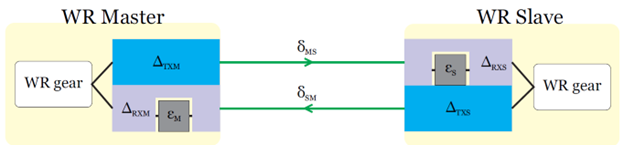
\includegraphics  {my_folder/images//conn_model}
	\caption{Модель соединения между двумя устройствами} 
	\label{fig:conn-model}  
\end{figure}

На \firef{fig:conn-model} изображены возникающие задержки, требующие калибровки. Внутри каждого устройства 
возникают задержки на приёме и отправке ($\Delta_{TXM},\Delta_{RXM},\Delta_{TXS},\Delta_{RXS}, \varepsilon_{M},\varepsilon_{S}$),
которые являются результатом задержек в SFP (Small Form-factor Pluggable) 
модуле, в электрических цепях и электронных компонентах. Эти задержки калибруются отдельно на каждом устройстве и не являются
предметом рассмотрения в данной работе.

Суммарная задержка распространения сигнала от ведущего устройства к ведомому устройству и обратно считается по формуле:

\begin{equation}
delay_{MM} = \Delta_{TXM} + \Delta_{RXS} + \varepsilon_{S} + \Delta_{TXS} + \Delta_{RXM} + \varepsilon_{M} + \delta_{MS} + \delta_{SM}
\end{equation}

В данной работе рассматривается калибровка задержек $\delta_{MS}$ и $\delta_{SM}$ – задержек распространения сигнала по оптоволокну.

Когда оптоволокно ещё не установлено, измерить задержки и вычислить коэффициент асимметричности можно без особых усилий.
Коэффициент асимметричности определяется, как:

\begin{equation}
	\alpha = \frac{\delta_{MS} - \delta_{SM}}{\delta_{SM}}
\end{equation}

Измеряется коэффициент при помощи дополнительного короткого оптоволокна, с известной задержкой.

\begin{figure}[ht!] 
	\center
	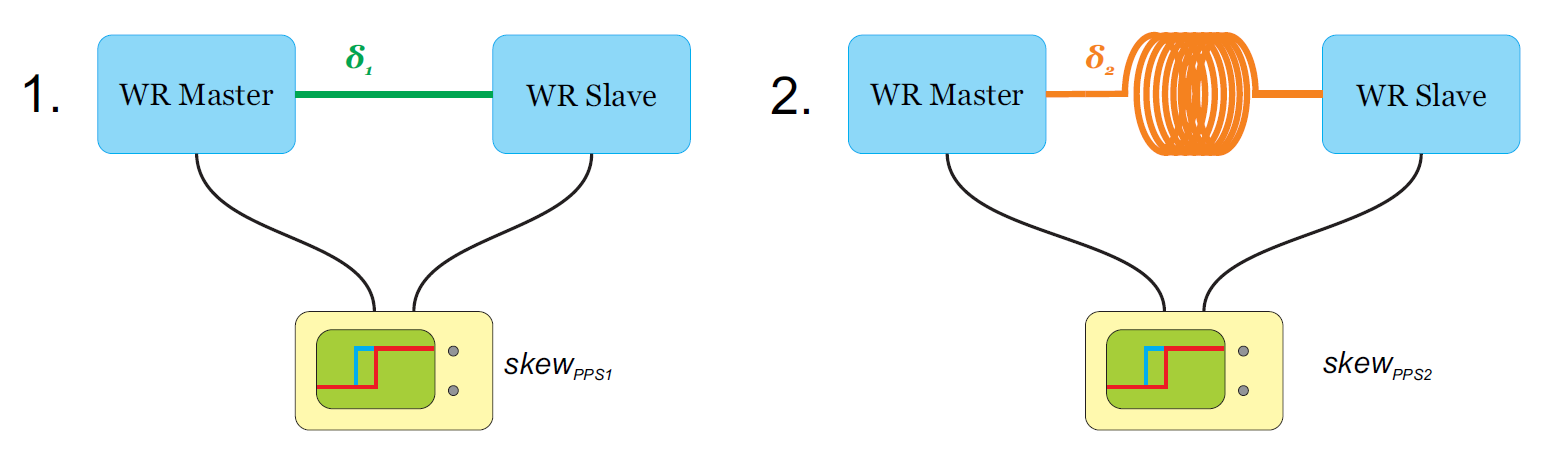
\includegraphics [scale=0.4] {my_folder/images//meas_scheme_1}
	\caption{Измерение асимметричности про помощи дополнительного оптоволокна} 
	\label{fig:meas-scheme-1}  
\end{figure}

Два устройства подключаются калибруемым оптоволокном ($\delta_{2}$) и дополнительным ($\delta_{1}$) отдельно, 
далее два устройства синхронизируются. После этого измеряется разность фаз синхросигналов 1-PPS
(Pulse Per Second), генерируемых ведущим и ведомым устройством. 

\begin{equation}
	skew_{PPS} = t_{PPS_S} - t_{PPS_M}
\end{equation}

По измеренным значениям можно определить коэффициент асимметричности, как:

\begin{equation}
	\alpha = \frac{2 \left( skew_{PPS2} - skew_{PPS1} \right) }{\frac{1}{2} \delta_2 - \left( skew_{PPS2} - skew_{PPS1} \right)}
\end{equation}






\subsection{Название первого подпараграфа первого параграфа первой главы для~демонстрации переноса слов в содержании} % ~ нужен, чтобы избавиться от висячего предлога (союза) в конце строки

Содержание первого подпараграфа первого параграфа первой главы.



Одиночные формулы оформляют в окружении \texttt{equation}, например, как указано в следующей одиночной нумерованной формуле:
%
%
\begin{equation}% лучше не оставлять пропущенную строку (\par) перед окружениями для избежания лишних отсупов в pdf
\label{eq:Pi-ch1} % eq - equations, далее название, ch поставлено для избежания дублирования
\pi \approx 3,141.
\end{equation}
%
%
\begin{figure}[ht!] 
	\center
	\includegraphics [scale=0.27] {my_folder/images//spbpu_hydrotower}
	\caption{Вид на гидробашню СПбПУ \cite{spbpu-gallery}} 
	\label{fig:spbpu_hydrotower}  
\end{figure}
%
%
%\begin{table} [htbp]% Пример оформления таблицы
%	\centering\small
%	\caption{Представление данных для сквозного примера по ВКР \cite{Peskov2004}}%
%	\label{tab:ToyCompare}		
%		\begin{tabular}{|l|l|l|l|l|l|}
%			\hline
%			$G$&$m_1$&$m_2$&$m_3$&$m_4$&$K$\\
%			\hline
%			$g_1$&0&1&1&0&1\\ \hline
%			$g_2$&1&2&0&1&1\\ \hline
%			$g_3$&0&1&0&1&1\\ \hline
%			$g_4$&1&2&1&0&2\\ \hline
%			$g_5$&1&1&0&1&2\\ \hline
%			$g_6$&1&1&1&2&2\\ \hline		
%		\end{tabular}	
%	\normalsize% возвращаем шрифт к нормальному
%\end{table}


% \firef{} от figure reference
% \taref{} от table reference
% \eqref{} от equation reference

На \firef{fig:spbpu_hydrotower} изображена гидробашня СПбПУ, а в \taref{tab:ToyCompare} приведены данные, на примере которых коротко и наглядно будет изложена суть ВКР.


\section{Название параграфа} \label{ch1:sec2} 



Формулы могут быть размещены в несколько строк. Чтобы выставить номер формулы напротив средней строки, используйте окружение \verb|multlined| из пакета \verb|mathtools| следующим образом \cite{Ganter1999}:
%
\begin{equation} 
\label{eq:fConcept-order-ch1}
\begin{multlined}
(A_1,B_1)\leq (A_2,B_2)\; \Leftrightarrow \\  \Leftrightarrow\; A_1\subseteq A_2\; \Leftrightarrow \\ \Leftrightarrow\; B_2\subseteq B_1. 
\end{multlined}
\end{equation}


Используя команду \verb|\labelcref| из пакета \verb|cleveref|, допустимо следующим образом оформлять ссылку на несколько формул:
(\labelcref{eq:Pi-ch1,eq:fConcept-order-ch1}).
%
%
\input{my_folder/tex/fig-spbpu-whitehall-three-in-one} % пример подключения 3х иллюстрации в одном рисунке

Пример ссылок \cite{Article,Book,Booklet,Conference,Inbook,Incollection,Manual,Mastersthesis,Misc,Phdthesis,Proceedings,Techreport,Unpublished,badiou:briefings}, а также ссылок с указанием страниц, на котором отображены номера страниц  \cite[с.~96]{Naidenova2017} или в виде мультицитаты на несколько источников \cites[с.~96]{Naidenova2017}[с.~46]{Ganter1999}. Часть библиографических записей носит иллюстративный характер и не имеет отношения к реальной литературе. 



%\FloatBarrier % заставить рисунки и другие подвижные (float) элементы остановиться

\section{Выводы} \label{ch1:conclusion}

Текст выводов по главе \thechapter.

Кроме названия параграфа <<выводы>> можно использовать (единообразно по всем главам) следующие подходы к именованию последних разделов с результатами по главам:
\begin{itemize}
	\item <<выводы по главе N>>, где N --- номер соответствующей главы;
	\item <<резюме>>;
	\item <<резюме по главе N>>, где N --- номер соответствующей главы.
\end{itemize}

Параграф с изложением выводов по главе \textit{является обязательным}.

%% Вспомогательные команды - Additional commands
%
%\newpage % принудительное начало с новой страницы, использовать только в конце раздела
%\clearpage % осуществляется пакетом <<placeins>> в пределах секций
%\newpage\leavevmode\thispagestyle{empty}\newpage % 100 % начало новой страницы